% Options for packages loaded elsewhere
\PassOptionsToPackage{unicode}{hyperref}
\PassOptionsToPackage{hyphens}{url}
\PassOptionsToPackage{dvipsnames,svgnames,x11names}{xcolor}
\documentclass[
  11pt,
  onecolumn]{article}
\usepackage{xcolor}
\usepackage[margin=2cm]{geometry}
\usepackage{amsmath,amssymb}
\setcounter{secnumdepth}{-\maxdimen} % remove section numbering
\usepackage{iftex}
\ifPDFTeX
  \usepackage[T1]{fontenc}
  \usepackage[utf8]{inputenc}
  \usepackage{textcomp} % provide euro and other symbols
\else % if luatex or xetex
  \usepackage{unicode-math} % this also loads fontspec
  \defaultfontfeatures{Scale=MatchLowercase}
  \defaultfontfeatures[\rmfamily]{Ligatures=TeX,Scale=1}
\fi
\usepackage{lmodern}
\ifPDFTeX\else
  % xetex/luatex font selection
\fi
% Use upquote if available, for straight quotes in verbatim environments
\IfFileExists{upquote.sty}{\usepackage{upquote}}{}
\IfFileExists{microtype.sty}{% use microtype if available
  \usepackage[]{microtype}
  \UseMicrotypeSet[protrusion]{basicmath} % disable protrusion for tt fonts
}{}
\usepackage{setspace}
\makeatletter
\@ifundefined{KOMAClassName}{% if non-KOMA class
  \IfFileExists{parskip.sty}{%
    \usepackage{parskip}
  }{% else
    \setlength{\parindent}{0pt}
    \setlength{\parskip}{6pt plus 2pt minus 1pt}}
}{% if KOMA class
  \KOMAoptions{parskip=half}}
\makeatother
\usepackage{longtable,booktabs,array}
\newcounter{none} % for unnumbered tables
\usepackage{calc} % for calculating minipage widths
% Correct order of tables after \paragraph or \subparagraph
\usepackage{etoolbox}
\makeatletter
\patchcmd\longtable{\par}{\if@noskipsec\mbox{}\fi\par}{}{}
\makeatother
% Allow footnotes in longtable head/foot
\IfFileExists{footnotehyper.sty}{\usepackage{footnotehyper}}{\usepackage{footnote}}
\makesavenoteenv{longtable}
\usepackage{graphicx}
\usepackage{wrapfig}
\usepackage{subcaption}
\makeatletter
\newsavebox\pandoc@box
\newcommand*\pandocbounded[1]{% scales image to fit in text height/width
  \sbox\pandoc@box{#1}%
  \Gscale@div\@tempa{\textheight}{\dimexpr\ht\pandoc@box+\dp\pandoc@box\relax}%
  \Gscale@div\@tempb{\linewidth}{\wd\pandoc@box}%
  \ifdim\@tempb\p@<\@tempa\p@\let\@tempa\@tempb\fi% select the smaller of both
  \ifdim\@tempa\p@<\p@\scalebox{\@tempa}{\usebox\pandoc@box}%
  \else\usebox{\pandoc@box}%
  \fi%
}
% Set default figure placement to htbp
\def\fps@figure{htbp}
\makeatother
\setlength{\emergencystretch}{3em} % prevent overfull lines
\providecommand{\tightlist}{%
  \setlength{\itemsep}{0pt}\setlength{\parskip}{0pt}}
\usepackage{bookmark}
\IfFileExists{xurl.sty}{\usepackage{xurl}}{} % add URL line breaks if available
\urlstyle{same}
\hypersetup{
  colorlinks=true,
  linkcolor={blue},
  filecolor={Maroon},
  citecolor={Blue},
  urlcolor={blue},
  pdfcreator={LaTeX via pandoc}}

\author{}
\date{}

\begin{document}

\begin{titlepage}
\centering
\newcommand{\HRule}{\rule{\linewidth}{0.5mm}}

\textsc{\LARGE University of New South Wales}\\[1.5cm]
% \textsc{\Large COMP9417 - Project}\\[0.5cm]

\HRule \\[0.4cm]
{\huge \bfseries COMP9417 - Group Project - xRFM}\\[0.4cm]
\HRule \\[1.5cm]

\includegraphics[scale=0.6]{logo.PNG}\\[1cm]

\textbf{Group:} Twinkle Twinkle\\[0.5cm]

\begin{tabular}{c|c}
John Zhang        & z5591121 \\
Shaohua Wang      & z5489497 \\
Zian Hu        & z5514488 \\
Yonje Ryu & z5338581 \\
\end{tabular}

\vfill
\end{titlepage}

\setstretch{1.35}

\subsection{1. Introduction}\label{introduction}

Tabular data resists deep learning: targets jump abruptly along feature
axes, scales are heterogeneous, and many columns are uninformative;
gradient-boosted decision trees (GBDTs) handle these properties naturally
{[}Grinsztajn et al., 2022{]}. Classical kernel methods don't displace
them either: kernels fix feature similarity \emph{before} training (so
they cannot learn which features matter), and kernel ridge regression
costs \(O(n^3)\), intractable above \textasciitilde70k samples.

\textbf{xRFM} {[}Beaglehole et al., 2025{]} tackles both. An inner
Recursive Feature Machine {[}Radhakrishnan et al., 2024{]} learns the
Average Gradient Outer Product (AGOP), a matrix of per-input
sensitivities, and reshapes the kernel through it. An outer balanced
binary tree splits along the top AGOP eigenvector of a local RFM,
bringing training to \(O(n \log n)\) and producing a per-leaf AGOP for
subpopulation interpretability. We test xRFM on five UCI datasets (none
in the TALENT benchmark or xRFM's meta-test suite) against XGBoost,
Random Forest, and CatBoost. xRFM is competitive on smooth-target tasks
(Appliances Energy, Crop Mapping), trails on rule-like and small-\(n\)
problems (Seoul Bike, HCC), and is more hyperparameter-sensitive on
imbalanced high-dimensional data (IDA2016).

\subsection{2. Methodology}\label{methodology}

\subsubsection{2.1 Average Gradient Outer Product
(AGOP)}\label{average-gradient-outer-product-agop}

AGOP is the matrix at the heart of xRFM's feature learning: across
training points, in which input directions does the model's prediction
change most? For a trained predictor
\(\hat f: \mathbb{R}^d \to \mathbb{R}\) and training set
\(\mathcal{S} = \{x^{(1)}, \ldots, x^{(n)}\}\), AGOP is computed by
taking the gradient of \(\hat f\) at every training point, then
averaging the outer products:

\[
\mathrm{AGOP}(\hat f, \mathcal{S}) \;=\; \frac{1}{n}\sum_{i=1}^{n} \nabla \hat f\!\bigl(x^{(i)}\bigr)\,\nabla \hat f\!\bigl(x^{(i)}\bigr)^{\!\top} \;\in\; \mathbb{R}^{d\times d}. \tag{1}
\]

For any unit vector \(v\), the quadratic form \(v^\top M v\) measures
how strongly \(\hat f\) responds when its input moves along direction
\(v\). Two readouts of \(M\) answer different questions:

\begin{itemize}
\tightlist
\item
  \textbf{Diagonal entries \(M_{ii}\)} give per-feature sensitivity. A
  large \(M_{ii}\) means the model's output changes sharply when feature
  \(i\) changes, keeping the others fixed.
\item
  \textbf{Top eigenvectors of \(M\)} give the directions in feature
  space that the model actually uses (the \emph{active subspace} of
  Constantine et al., 2014). The top eigenvector \(v_1\) is a signed
  linear combination of features (positive and negative loadings push
  the prediction in opposite directions), capturing \emph{joint}
  structure that the diagonal alone misses.
\end{itemize}

\textbf{How AGOP compares to other importance methods.} \emph{PCA}
finds high-variance directions of \(x\) but ignores \(y\), so its
directions need not be predictive. \emph{Mutual information}
\(I(X_i; Y)\) is model-free and per-feature interpretable but cannot
capture joint structure. \emph{Permutation importance} shuffles a
feature and measures the loss change; intuitive but degrades under
correlated features. AGOP is supervised (depends on \(\hat f\)), joint
(off-diagonal entries encode interactions), and computed in a single
forward/backward pass; the cost is that it inherits the model's biases:
if \(\hat f\) overfits noise, AGOP assigns it apparent importance.

\subsubsection{2.2 The xRFM Algorithm}\label{the-xrfm-algorithm}

xRFM nests an iterative kernel-ridge RFM inside the leaves of a balanced
binary tree whose internal splits use an AGOP-based supervised
criterion.

\textbf{Tree construction.} Given a node with more than
\(L_{\max}\) points, xRFM trains a small RFM on a subsample and takes
the top eigenvector \(v_1\) of the local AGOP as the split direction:
every point is projected onto \(v_1\) and split at the
\textbf{median}, recursing until every leaf has at most \(L_{\max}\)
points. Median splits keep the tree balanced (depth \(O(\log n)\)),
which is the design choice distinguishing xRFM from prior AGOP-based trees and
the source of its \(O(n \log n)\) training cost.

\textbf{Leaf training.} At each leaf, an RFM is fitted using
the generalised kernel \(K_{p,q}(x, x') = \exp(-\|x - x'\|_p^q / L^q)\)
(Schoenberg, 1942) for \(0 < q \le p \le 2\). Two cases matter for our
experiments: \(q = 2\) recovers the rotation-invariant Laplace kernel
(the library's \texttt{l2} mode), and \(q = p\) gives an axis-aligned
product kernel (\texttt{l1}). Starting with \(M_0 = I\), the RFM
iteration alternates kernel-ridge fitting on inputs reshaped by
\(M_t^{1/2}\) with AGOP recomputation and normalisation, for up to
\(\tau \le 10\) rounds; we retain the iterate with the lowest
\emph{validation} error.

\textbf{Inference.} A test point \(x^\star\) is routed through the tree
(hard or soft median thresholds) to its leaf \(\ell\), then predicted as
\(\hat y = K(x^\star \odot M_\ell^{1/2}, X_{M_\ell}) \alpha_\ell\). A
single tree, with one predictor per test point and no ensembling.

\textbf{Computational complexity.} Training is \(O(n \log n)\): leaves
cap per-leaf cost at \(O(L_{\max}^3)\) (constant in \(n\)), and median
splits visit \(O(n)\) points at each of \(O(\log n)\) tree levels.
Inference is \(O(\log n + L_{\max})\) per sample. A naive kernel method
costs \(O(n^3)\) training and \(O(n^2)\) memory, which becomes
intractable above roughly 70,000 samples on a 40 GB GPU.

\subsubsection{2.3 Experimental Design}\label{experimental-design}

\textbf{Datasets.} Five UCI datasets (Table 1), absent from both the
TALENT benchmark and xRFM's meta-test suite. The selection spans stress
points for kernel methods: smooth-target regression (Appliances, Crop
Mapping), rule-like targets (Seoul Bike), small-\(n\) high-\(d/n\) with
missingness (HCC), and severe class imbalance (IDA2016,
\textasciitilde1.6\% positive). Appliances doubles as the
interpretability testbed (ships with two ground-truth noise features,
\texttt{rv1}/\texttt{rv2}).

\begin{center}
\begin{tabular}{@{}clrrll@{}}
\toprule
\# & Dataset (UCI ID) & \(n\) & \(d\) & Task & Features \\
\midrule
1 & Seoul Bike Sharing (560)     & 8,760  & 12  & Regression     & 9 num + 3 cat \\
2 & Appliances Energy (374)      & 19,735 & 27  & Regression     & All numeric \\
3 & HCC Survival (423)           & 165    & 49  & Binary         & 22 num + 27 cat \\
4 & IDA2016 Scania APS (414)     & 60,000 & 170 & Binary         & All numeric \\
5 & Crop Mapping, Winnipeg (525) & 50,000 & 174 & Multiclass (7) & All numeric \\
\bottomrule
\end{tabular}
\end{center}

\textbf{Splits.} Stratified 60/20/20 train/val/test with
\texttt{random\_state=42} (stratified on target for classification,
random for regression).

\textbf{Preprocessing.} Median imputation for numerics, mode imputation
for categoricals. For kernel methods (xRFM): standard-scaled numerics +
one-hot-encoded categoricals. For tree ensembles: numerics plus
ordinal-encoded categoricals (no standardisation, preserving split
structure). CatBoost receives native categorical indices.

\textbf{Hyperparameter tuning.} Optuna TPE sampler optimises the
validation-split primary metric (RMSE for regression, AUC-ROC for
binary, accuracy for multiclass) with model-specific trial budgets
(xRFM 25, XGBoost 40, CatBoost 30, Random Forest 20). xRFM gets fewer
trials because each kernel-ridge solve is the wall-clock bottleneck.
The configuration with the best validation objective is retrained on
the train split and evaluated once on held-out test. Full search
spaces, fixed knobs, and per-dataset selected HPs are in Appendix B.
Note that \texttt{max\_leaf\_size = min(60000, n\_train)} forces xRFM
into a single-leaf-RFM regime on all five main-comparison datasets;
the tree component is engaged only in the §3.2 interpretability run
(2 leaves on Appliances) and at \(n=36k\) in §3.3.

\textbf{Metrics.} Regression: RMSE (primary) and \(R^2\).
Classification: Accuracy and AUC-ROC (macro-OvR for multiclass). Plus
wall-clock training time and per-sample inference time.

\subsection{3. Results}\label{results}

\subsubsection{3.1 Main comparison}\label{main-comparison}

\textbf{Table 2. Final test-set results across all five datasets and
four models. Regression: lower RMSE is better. Classification: higher
Acc/AUC is better. Train is wall-clock training time (s); Inf is
per-sample inference time (µs). Best per dataset in bold; ties broken by
AUC for binary, Accuracy for multiclass.}

\begingroup\footnotesize

{\def\LTcaptype{none} % do not increment counter
\begin{longtable}[]{@{}
  >{\raggedright\arraybackslash}p{(\linewidth - 10\tabcolsep) * \real{0.20}}
  >{\raggedleft\arraybackslash}p{(\linewidth - 10\tabcolsep) * \real{0.10}}
  >{\raggedleft\arraybackslash}p{(\linewidth - 10\tabcolsep) * \real{0.175}}
  >{\raggedleft\arraybackslash}p{(\linewidth - 10\tabcolsep) * \real{0.175}}
  >{\raggedleft\arraybackslash}p{(\linewidth - 10\tabcolsep) * \real{0.175}}
  >{\raggedleft\arraybackslash}p{(\linewidth - 10\tabcolsep) * \real{0.175}}@{}}
\toprule\noalign{}
\begin{minipage}[b]{\linewidth}\raggedright
Dataset
\end{minipage} & \begin{minipage}[b]{\linewidth}\raggedright
Metric
\end{minipage} & \begin{minipage}[b]{\linewidth}\raggedleft
xRFM
\end{minipage} & \begin{minipage}[b]{\linewidth}\raggedleft
XGBoost
\end{minipage} & \begin{minipage}[b]{\linewidth}\raggedleft
CatBoost
\end{minipage} & \begin{minipage}[b]{\linewidth}\raggedleft
RF
\end{minipage} \\
\midrule\noalign{}
\endhead
\bottomrule\noalign{}
\endlastfoot
Appliances Energy & RMSE/R² & \textbf{65.29/0.574} & 65.75/0.568 &
66.96/0.552 & 72.61/0.473 \\
& Train/Inf & 11.5/26 & 41.7/95 & 11.1/\textbf{3.5} & \textbf{1.7}/41 \\
Seoul Bike & RMSE/R² & 238.44/0.864 & 232.32/0.870 &
\textbf{225.66/0.878} & 245.64/0.855 \\
& Train/Inf & 2.1/16 & 5.4/37 & 5.2/\textbf{1.9} & \textbf{0.5}/57 \\
\midrule
HCC Survival & Acc/AUC & 0.758/0.800 & 0.818/0.835 & 0.788/0.819 &
\textbf{0.849/0.850} \\
& Train/Inf & 0.1/50 & \textbf{0.0}/\textbf{19} & 0.6/47 & 0.9/3667 \\
IDA2016 & Acc/AUC & 0.990/0.990 & 0.993/\textbf{0.993} &
\textbf{0.994}/0.992 & 0.992/0.989 \\
& Train/Inf & 16.9/5.9 & 52.1/30 & \textbf{3.1}/\textbf{0.5} & 5.8/15 \\
Crop Mapping & Acc/AUC & \textbf{0.995/1.000} & 0.991/1.000 & n/a &
0.989/1.000 \\
& Train/Inf & 12.8/\textbf{2.6} & 40.0/20 & n/a & \textbf{12.2}/24 \\
\end{longtable}
}

\endgroup

\emph{Seeds fixed at 42. TabPFN-v2 omitted throughout (see §4 for
rationale). CatBoost on Crop Mapping timed out on our 2-hour Modal
budget at 7-class × 30k × 174-feature scale; other three models
converge.}

Tuning chose \texttt{kernel=l1} (axis-aligned) for the two lowest-\(d\)
datasets (Appliances, Seoul Bike) and \texttt{kernel=l2}
(rotation-invariant) for the three higher-\(d\) datasets (HCC, IDA2016,
Crop Mapping); per-dataset HPs are in Appendix B.

\textbf{xRFM is competitive on smooth-target tasks.} On Appliances
Energy it obtains the best RMSE in this single split, but the margin
over XGBoost is small (65.29 vs 65.75) and should not be
over-interpreted without multi-seed error bars. On Crop Mapping, xRFM
is best among the completed models, but CatBoost timed out, so this is
not evidence that xRFM dominates all GBDT baselines.
\textbf{GBDTs win on rule-like Seoul Bike} (CatBoost leads,
all four within 9\%; zero rentals when the system is off, and season ×
hour interactions favour splits) \textbf{and small-\(n\) HCC} (RF leads
xRFM by 9 accuracy
points; with 33 test samples, differences under \(\pm 6\) points
aren't significant at 5\%).

\subsubsection{3.2 Interpretability on Appliances
Energy}\label{interpretability-on-appliances-energy}

We compare AGOP from the tuned xRFM (\texttt{kernel=l1, diag=True})
against PCA loadings (unsupervised), mutual information (model-free
supervised), and signed permutation importance on an XGBoost proxy
(black-box supervised). \texttt{diag=True} restricts AGOP to per-feature
sensitivities; signed-eigenvector analysis (Fig. 7C) needs
\texttt{diag=False}, deferred.

\begin{figure}
\centering
\includegraphics[width=0.75\linewidth,keepaspectratio,alt={Feature importance comparison on Appliances Energy. {[}*{]} marks the two injected random features.}]{../figures/interpretability_appliances.png}
\caption{\footnotesize Feature importance comparison on Appliances
Energy (top-15 features by AGOP). {[}*{]} marks the two injected random
features.}
\end{figure}

\textbf{The random-feature test.} Out of \(d=27\) features, MI ranks
\texttt{rv1}, \texttt{rv2} at 26/27 and 27/27 and signed permutation at
27/27 and 26/27, so both cleanly identify the noise. AGOP places them
at 21/27 and 20/27, correct in direction but less decisive. PCA fails
outright at \textbf{2/27 and 1/27} (wrongly at the top), because random
uniforms are statistically independent of the correlated sensor
readings and so dominate input covariance. AGOP's noise rejection also
depends on the kernel fit: re-running with default HPs
(\texttt{bandwidth=10, kernel=l2, diag=False}) drops \texttt{rv1},
\texttt{rv2} to ranks 12--13, a nine-position degradation.

\begin{figure}[!ht]
\centering
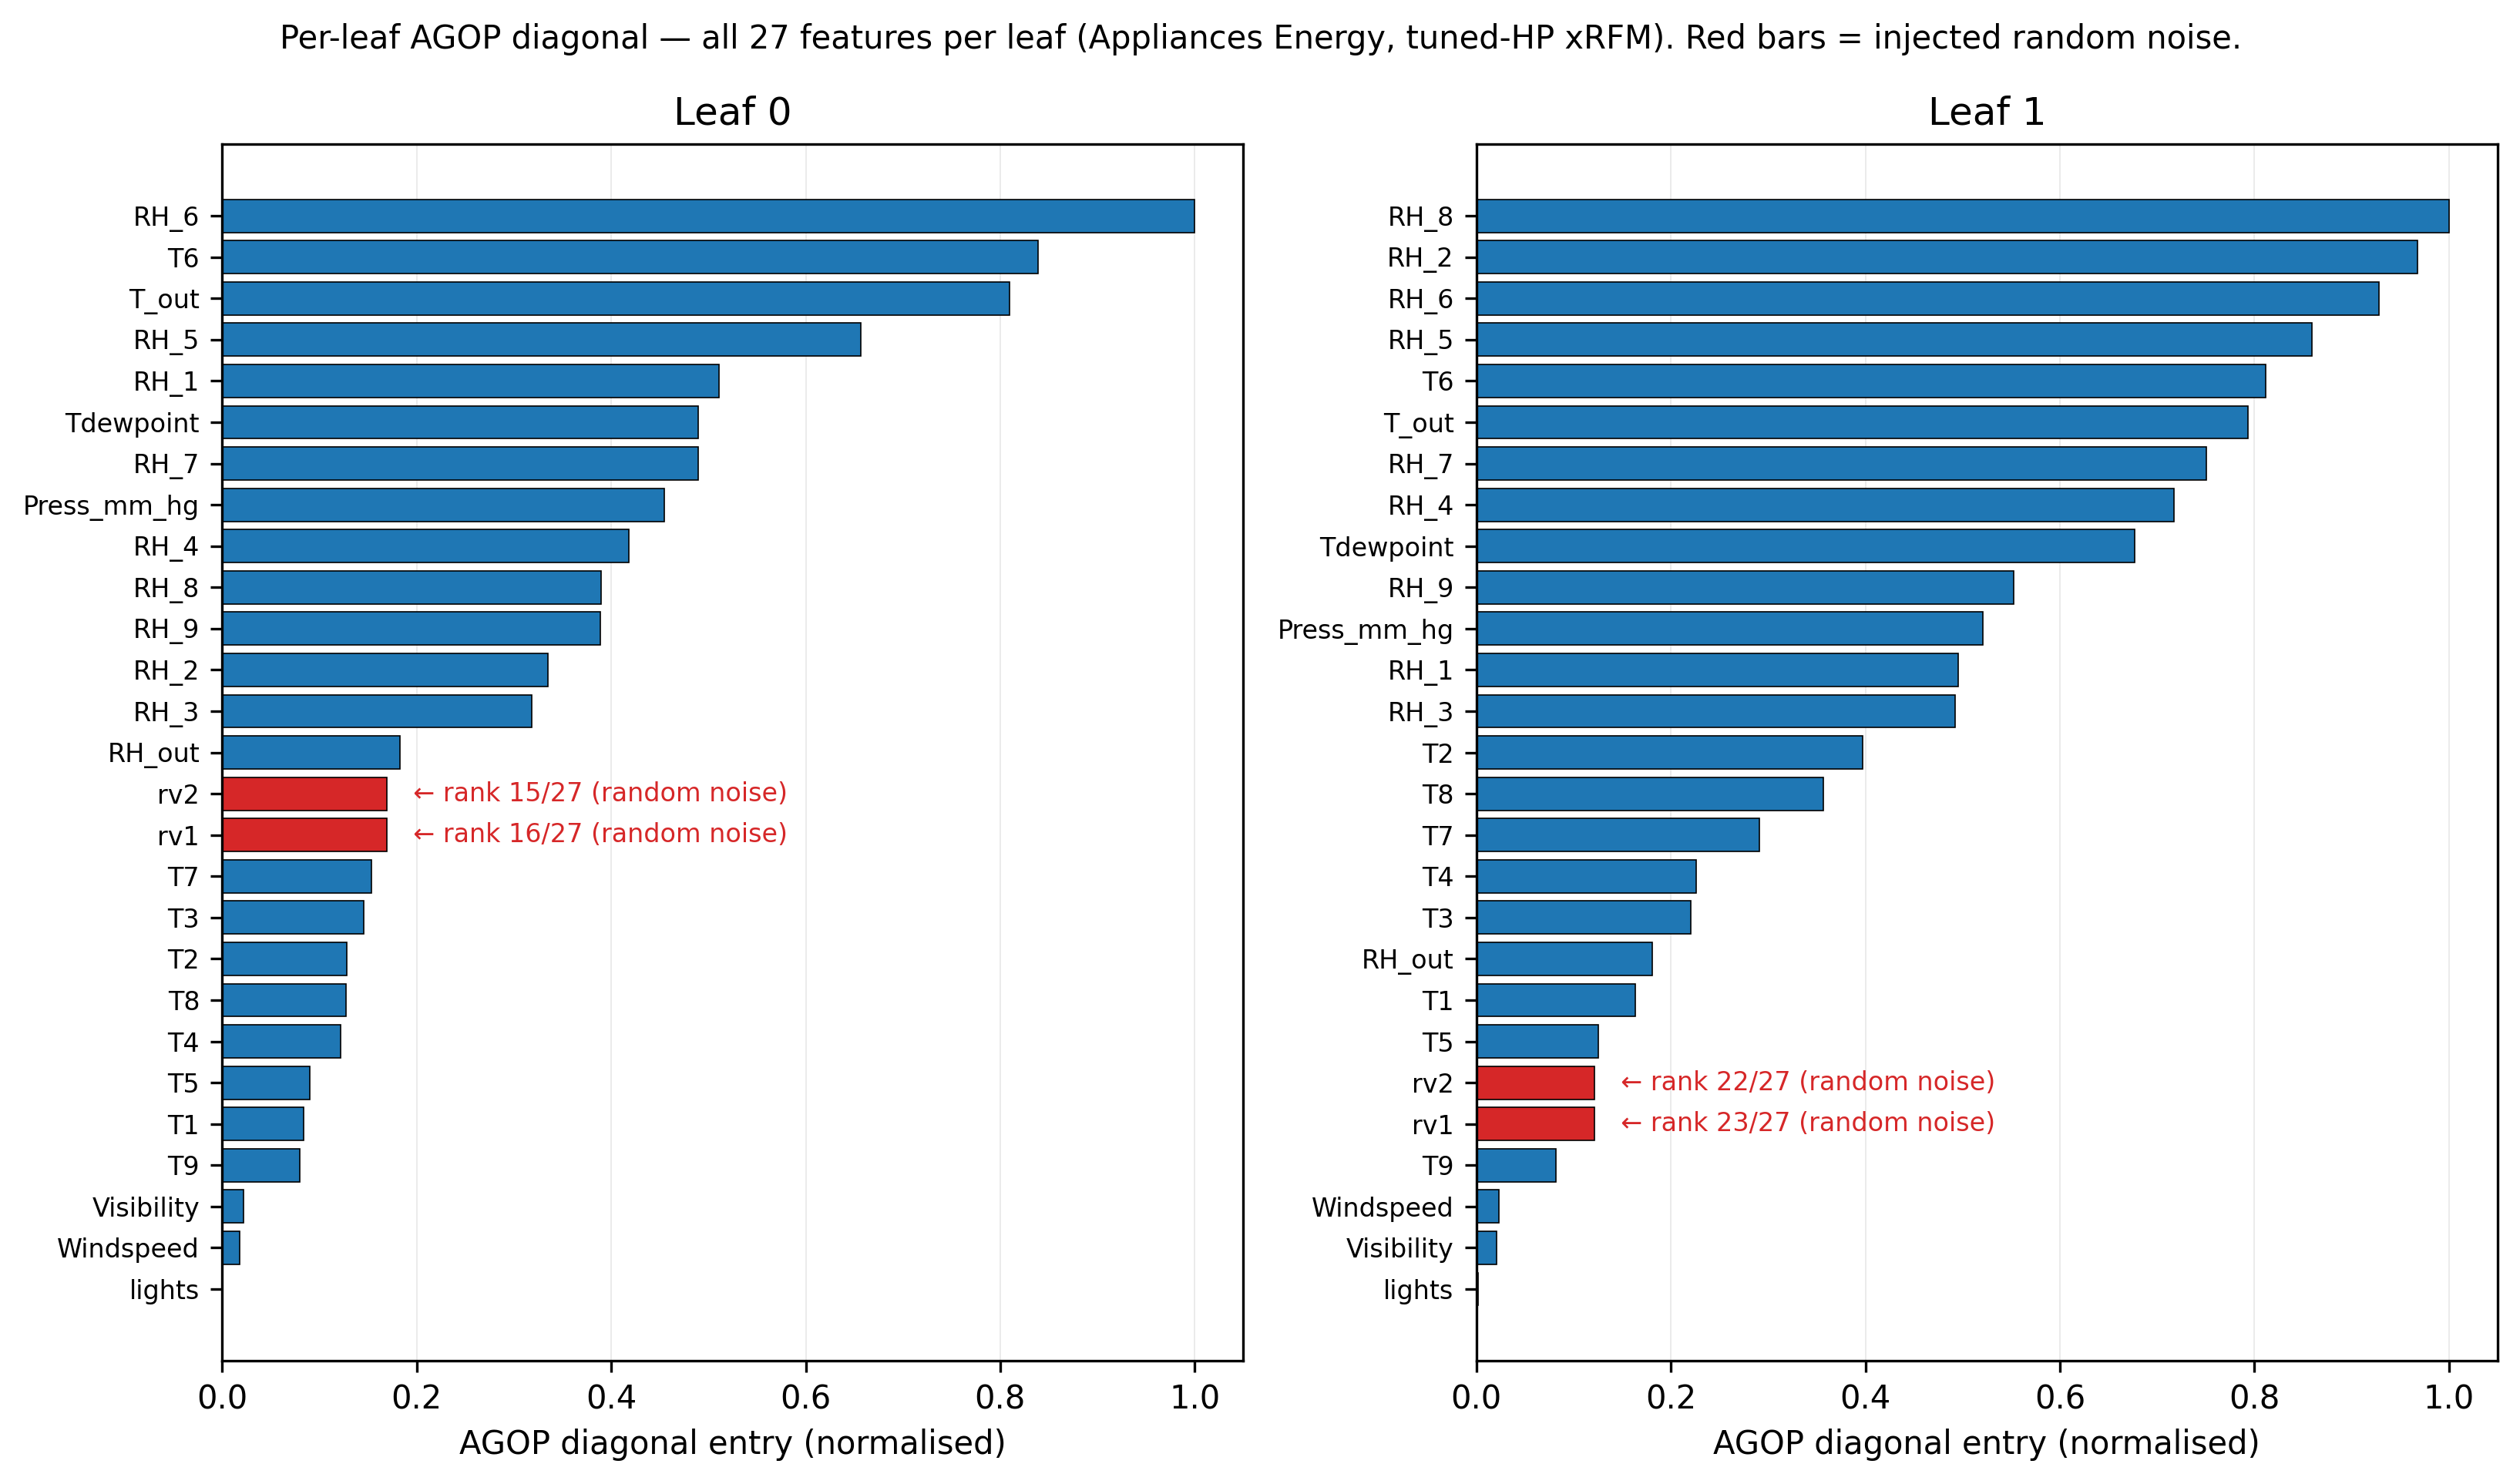
\includegraphics[width=0.7\linewidth,keepaspectratio,alt={Per-leaf AGOP diagonal for the tuned-HP xRFM. The two leaves identify different humidity sensors as locally most important: RH\_6 in leaf 0 and RH\_8 in leaf 1.}]{../figures/per_leaf_agop_appliances.png}
\caption{\footnotesize Per-leaf AGOP diagonal for the tuned-HP xRFM.
The two leaves identify different humidity sensors as locally most
important: RH\_6 in leaf 0 and RH\_8 in leaf 1.}
\end{figure}

\textbf{Per-leaf subpopulation structure.} The tuned tree has two
leaves; AGOP reveals different locally-relevant humidity sensors per
leaf: leaf 0 weights RH\_6 (kitchen) maximally (AGOP \(= 1.00\)),
leaf 1 weights RH\_8 (parents' room) maximally, mirroring the per-leaf
specialisation Beaglehole et al.~(2025, Fig. 7B) report for NYC Taxi.
T6 (outdoor) and RH\_5 (bathroom) rank high in both. With only 2 leaves
the effect is small-scale; deeper trees on larger datasets would
amplify it. Per-leaf \texttt{rv1}/\texttt{rv2} ranks are 15--16/27 in
leaf 0 and 22--23/27 in leaf 1, so noise demotion strengthens with
deeper splits.

AGOP and signed permutation also agree on which real features matter:
four of permutation's top-5 (RH\_4, RH\_2, RH\_8, T4) appear in AGOP's
top-10, both highlighting indoor humidity over outdoor temperature.

\subsubsection{3.3 Scaling study on
IDA2016}\label{scaling-study-on-ida2016}

Figure 3 plots test AUC-ROC and training time against subsampled
training size \(n \in \{1k, 2.5k, 5k, 10k, 20k, 36k\}\) with the test set
held fixed. Unlike the earlier default-HP sweep, this rerun freezes each
model's Optuna-selected full-\(n\) hyperparameters from §3.1 and refits
preprocessing on each subsampled training set only. The AUC panel uses a
broken y-axis so the XGBoost \(n=1k\) chance-level point remains visible
while the \(0.98+\) comparison band is readable. This better isolates the
effect of training-set size than the default-HP sweep, but it is still
single-seed and should not be read as an asymptotic complexity test.

\begin{figure}[!ht]
\centering
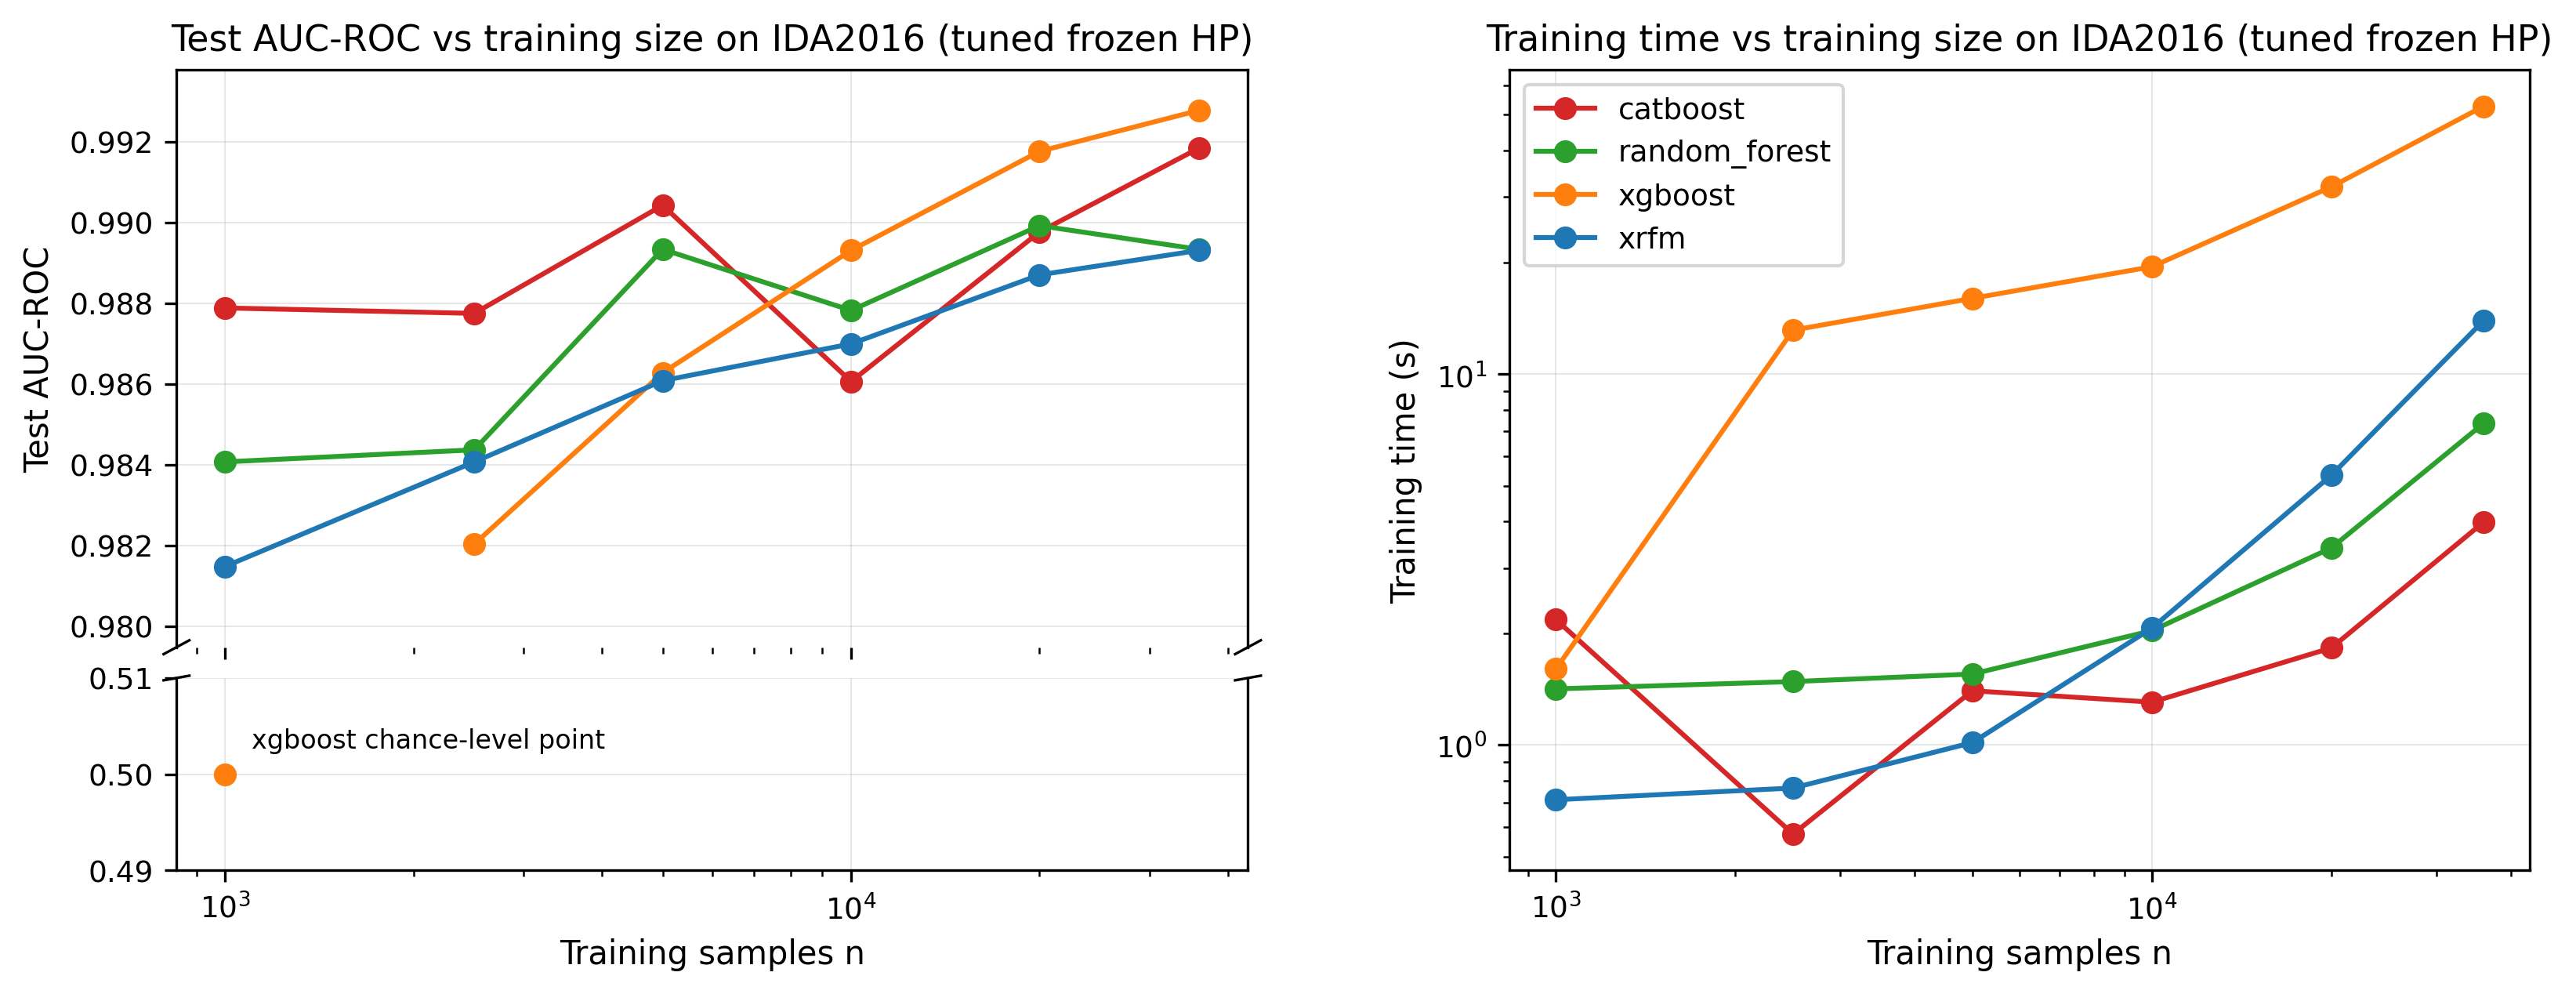
\includegraphics[width=1\linewidth,height=\textheight,keepaspectratio,alt={Test AUC-ROC with broken y-axis (left) and training time (right) vs.~training size on IDA2016 with full-n tuned hyperparameters frozen.}]{../figures/scaling_ida2016_tuned.png}
\caption{\footnotesize Test AUC-ROC with broken y-axis (left) and
training time (right) vs.~training size on IDA2016 with full-\(n\)
tuned hyperparameters frozen.}
\end{figure}

\begin{enumerate}
\def\labelenumi{\arabic{enumi}.}
\tightlist
\item
  \textbf{Tuned sample scaling.} xRFM improves AUC from 0.981 (\(n=1k\))
  to 0.989 (\(n=36k\)), matching RF (0.989) but trailing CatBoost
  (0.992) and XGBoost (0.993). XGBoost's full-\(n\) tuned configuration
  fails at \(n=1k\) (AUC 0.500), showing frozen-HP scaling is
  configuration-specific.
\item
  \textbf{Tree engagement is shallow.} xRFM logs one leaf through
  \(n=20k\) and two at \(n=36k\) (the library rescales effective
  \texttt{max\_leaf\_size} to \(\approx\)26.6k); the sweep mostly
  measures leaf-RFM behaviour.
\item
  \textbf{Training time.} xRFM grows from 0.71 s (\(n=1k\)) to 13.93 s
  (\(n=36k\)); log-log slope 0.84. Faster than XGBoost (52.7 s) but
  slower than CatBoost (4.0 s) and RF (7.4 s) at full size; these are wall-clock
  measurements, not a complexity-claim test.
\end{enumerate}

\subsection{4. Discussion}\label{discussion}

\textbf{Theory alignment.} xRFM should be strongest on smoothly-varying
targets and weaker on rule-like ones where threshold splits are the
right inductive bias. The results are broadly consistent with this:
xRFM is highly competitive on Appliances Energy and Crop Mapping
(continuous sensors / 174 spectral bands), and loses narrowly on Seoul
Bike (sharp on/off rules, season × hour interactions). The surprise is
HCC Survival. Classical kernel theory predicts that kernels should do
well in small-\(n\) regimes via RKHS regularisation; instead Random
Forest beats xRFM by 9 accuracy points. Our hypothesis: with
\(n_\text{train}=99\), learning a \(108 \times 108\) AGOP matrix (the
encoded dimension after one-hot expansion of the 27 categorical
features) is statistically fragile, so noisy AGOP implies noisy
reweighting.

\textbf{xRFM is more hyperparameter-sensitive than the GBDTs.} IDA2016
makes this clearest: tuned xRFM reaches AUC 0.990 (within 0.3 of
CatBoost/XGBoost) but the earlier default-HP run gave only 0.978, a
1.2-point configuration effect. Three IDA2016 features match Grinsztajn et al.~(2022)'s kernel-loss predictions:
\begin{itemize}
\tightlist
\item
  \textbf{Class imbalance (1.6\% positive).} Kernel ridge minimises
  squared error symmetrically, with no minority up-weighting.
\item
  \textbf{170 dimensions, most low-signal.} xRFM must \emph{learn}
  relevance via AGOP; trees ignore noise via split selection.
\item
  \textbf{8.3\% missingness.} All models receive median-imputed numerics
  in our pipeline, so we did not test native tree missing-value
  handling; a defensible hypothesis is that median imputation distorts
  similarity geometry more for kernels than for split-based models.
\end{itemize}

\textbf{Choice of metrics.} We report RMSE rather than MAE for
regression because both Appliances Energy and Crop Mapping have
heavy-tailed targets where large errors deserve disproportionate
penalty; \(R^2\) accompanies RMSE for cross-dataset comparability since
target ranges differ by orders of magnitude (Appliances mean 97 Wh
vs.~Seoul Bike mean 705 rentals). For classification we report both
Accuracy and AUC-ROC, but on IDA2016 (1.6\% positive) AUC is the
load-bearing number, since accuracy \(\approx 0.984\) is trivially
achievable by always predicting ``no failure'', while AUC tests
rank-ordering of failure probabilities, so the fact that all four
models exceed 0.989 says they actually learn the rare class.
Train/inference times in Tables 2--3 are wall-clock on shared cloud
hardware with xRFM on GPU (CUDA) and the other three on CPU, so they
reflect hardware asymmetry and should not be read as a method-fair
complexity comparison.

\textbf{AGOP vs.~MI / permutation / PCA.} Our random-feature test
confirms §2.1's prediction that AGOP inherits model biases (tuned RFM
demotes noise to rank 20--21/27; default-HP RFM only 12--13/27); MI and
signed permutation sidestep this. Practical takeaway: \textbf{AGOP for
interpreting a tuned model, MI or signed permutation as a model-free
sanity check, PCA as a null baseline.}

\textbf{With more time.} Multi-seed replication (we used seed 42 only)
would put error bars on close comparisons, especially HCC's 33-sample
test. The HP search swept only \texttt{exponent} across two kernel
slices (\texttt{l1}, \texttt{l2}); the full \(K_{p,q}\) grid for
\(0 < q \le p \le 2\) is the natural follow-up. Smaller
\texttt{max\_leaf\_size} sweeps would test the partitioned-tree regime
our experiments only marginally entered.

\subsection{5. Conclusion}\label{conclusion}

xRFM is a credible complement to GBDTs in these experiments, especially
where AGOP interpretability is useful. On our five UCI datasets it is
competitive on smooth-target tasks (Appliances Energy, Crop Mapping),
improves substantially with HP tuning on imbalanced high-dimensional
classification (IDA2016), and trails on small-\(n\) (HCC) and rule-like
targets (Seoul Bike) where tree inductive bias is better matched.
However, the evidence is single-seed, only lightly exercises xRFM's tree
partitioning, and is not sufficient to establish robust superiority over
XGBoost or CatBoost.

\subsection{References}\label{references}

\begin{enumerate}
\def\labelenumi{\arabic{enumi}.}
\tightlist
\item
  Beaglehole, D., Holzmüller, D., Radhakrishnan, A., \& Belkin, M.
  (2025). \emph{xRFM: Accurate, scalable, and interpretable feature
  learning models for tabular data}. arXiv:2508.10053.
\item
  Radhakrishnan, A., Beaglehole, D., Pandit, P., \& Belkin, M. (2024).
  Mechanism for feature learning in neural networks and
  backpropagation-free machine learning models. \emph{Science},
  \textbf{383}(6690).
\item
  Chen, T., \& Guestrin, C. (2016). XGBoost: A scalable tree boosting
  system. In \emph{KDD 2016}.
\item
  Breiman, L. (2001). Random Forests. \emph{Machine Learning},
  \textbf{45}(1), 5--32.
\item
  Prokhorenkova, L., Gusev, G., Vorobev, A., Dorogush, A. V., \& Gulin,
  A. (2018). CatBoost: unbiased boosting with categorical features. In
  \emph{NeurIPS 2018}.
\item
  Hollmann, N., Müller, S., Purucker, L., Krishnakumar, A., Körfer, M.,
  Hoo, S. B., Schirrmeister, R. T., \& Hutter, F. (2025). Accurate
  predictions on small data with a tabular foundation model.
  \emph{Nature}, \textbf{637}.
\item
  Grinsztajn, L., Oyallon, E., \& Varoquaux, G. (2022). Why do
  tree-based models still outperform deep learning on typical tabular
  data? In \emph{NeurIPS 2022 Datasets \& Benchmarks Track}.
\item
  Ye, H.-J., Liu, S.-Y., Rong, H.-R., Lu, P.-X., Du, J.-Y., Chao, W.-L.,
  Wang, Z.-J., Sun, Q., \& Jiang, Y. (2024). \emph{A Closer Look at Deep
  Learning on Tabular Data (TALENT)}. arXiv:2407.00956.
\item
  Constantine, P. G., Dow, E., \& Wang, Q. (2014). Active subspace
  methods in theory and practice. \emph{SIAM J. Sci. Comput.},
  \textbf{36}(4).
\item
  Beaglehole, D., Súkeník, P., Mondelli, M., \& Belkin, M. (2024).
  Average gradient outer product as a mechanism for deep neural
  collapse. In \emph{NeurIPS 2024}.
\item
  Candanedo, L. M., Feldheim, V., \& Deramaix, D. (2017). Data driven
  prediction models of energy use of appliances in a low-energy house.
  \emph{Energy and Buildings}, \textbf{140}, 81--97.
\item
  Dua, D., \& Graff, C. (2017). UCI Machine Learning Repository.
  University of California, Irvine.
\item
  Akiba, T., Sano, S., Yanase, T., Ohta, T., \& Koyama, M. (2019).
  Optuna: A next-generation hyperparameter optimization framework. In
  \emph{KDD 2019}.
\end{enumerate}

\subsection{Appendix A: Dataset Feature
Descriptions}\label{appendix-a-dataset-feature-descriptions}

\subsubsection{A.1 Seoul Bike Sharing (UCI
560)}\label{a.1-seoul-bike-sharing-uci-560}

Hourly rental counts in Seoul, Sept 2017 -- Nov 2018 (\(n=8{,}760\),
\(d=12\)). Target: \texttt{Rented\_Bike\_Count} \(\in [0, 3556]\), mean
704.6, std 645.0. \textbf{No missing values.}

\begin{itemize}
\tightlist
\item
  \textbf{Numeric (9):} \texttt{Hour} (0--23), \texttt{TemperatureC}
  (−17.8 to 39.4), \texttt{Humiditypct} (0--98),
  \texttt{Wind\_speed\_m/s} (0--7.4), \texttt{Visibility\_10m}
  (27--2000), \texttt{Dew\_point\_temperatureC} (−30.6 to 27.2),
  \texttt{Solar\_Radiation\_MJ/m²} (0--3.52), \texttt{Rainfallmm}
  (0--35), \texttt{Snowfall\_cm} (0--8.8).
\item
  \textbf{Categorical (3):} \texttt{Seasons} (4 levels),
  \texttt{Holiday} (Yes/No), \texttt{Functioning\_Day} (Yes/No).
\end{itemize}

The target follows clear rules: rentals are exactly zero whenever the
bike system is off (\texttt{Functioning\_Day=No}); otherwise demand has
two daily peaks (morning and evening commutes); and the time-of-day
pattern depends strongly on the season. These are exactly the kind of
axis-aligned, piecewise-constant patterns that decision trees handle
naturally, which is a structural reason to expect GBDTs to do well here.

\subsubsection{A.2 Appliances Energy Prediction (UCI
374)}\label{a.2-appliances-energy-prediction-uci-374}

10-minute energy readings from a Belgian house (\(n=19{,}735\),
\(d=27\), all numeric). Target: \texttt{Appliances} (Wh)
\(\in [10, 1080]\), mean 97.7, std 102.5. \textbf{No missing values.}

\begin{itemize}
\tightlist
\item
  \textbf{Indoor sensors (18):} \texttt{T1}--\texttt{T9} (room
  temperatures, 14.9--29.9 °C), \texttt{RH\_1}--\texttt{RH\_9} (room
  humidities, 1--100\%).
\item
  \textbf{Outdoor weather (7):} \texttt{T\_out}, \texttt{Press\_mm\_hg},
  \texttt{RH\_out}, \texttt{Windspeed}, \texttt{Visibility},
  \texttt{Tdewpoint}, \texttt{lights}.
\item
  \textbf{Random noise (2):} \texttt{rv1}, \texttt{rv2}, both drawn from
  \(\mathcal{U}(0, 50)\) by Candanedo et al.~(2017) as
  ground-truth-irrelevant features. Used as the ``noise rejection''
  check in §3.2.
\end{itemize}

\subsubsection{A.3 HCC Survival (UCI
423)}\label{a.3-hcc-survival-uci-423}

Hepatocellular carcinoma 1-year survival in a Portuguese cohort
(\(n=165\), \(d=49\)). Target: binary survival outcome, \textbf{class
balance 102 lives : 63 dies (62\%/38\%)}. \textbf{826 missing values
(10.2\% of cells).} Features anonymised as \texttt{x0}--\texttt{x48}.

\begin{itemize}
\tightlist
\item
  \textbf{Categorical (27):} \texttt{x0}--\texttt{x22} are 22 binary
  clinical flags (cirrhosis, alcoholism, hepatitis, ascites, etc.);
  \texttt{x26} (5 levels: ECOG performance status),
  \texttt{x27}/\texttt{x28} (3 levels each: encephalopathy/ascites
  grades), \texttt{x43} (6 levels: Child-Pugh).
\item
  \textbf{Numeric (22):} Lab values with widely varying scales:
  \texttt{x23} (age, 20--93), \texttt{x30} (likely AFP, range 1.2 to
  1.8M), \texttt{x33}/\texttt{x34} (likely AST/ALT, max 13k and 459k
  respectively), plus haemoglobin, platelets, bilirubin, INR,
  creatinine, iron studies. Missingness up to 48\% on rarely-ordered
  tests.
\end{itemize}

High \(d/n \approx 0.30\), which is the report's primary hypothesis for
xRFM's underperformance on this dataset.

\subsubsection{A.4 IDA2016 Scania APS (UCI
414)}\label{a.4-ida2016-scania-aps-uci-414}

Heavy-truck Air Pressure System failure prediction (\(n=60{,}000\),
\(d=170\), all numeric). Target: binary (failure/no), \textbf{class
balance 59,000 : 1,000 (1.67\% positive).} \textbf{850,015 missing
values (8.3\% of cells).}

Features are anonymised sensor readings (\texttt{aa\_000},
\texttt{ab\_000}, \ldots); the \texttt{ag\_000}--\texttt{ag\_009} series
are histogram bins of one underlying counter. \textbf{Eight columns are
\textgreater50\% missing} (e.g., \texttt{br\_000} 82\%, \texttt{bq\_000}
81\%, \texttt{bp\_000} 80\%). All three properties stress kernel methods
specifically. With 170 mostly-uninformative dimensions, xRFM has to
\emph{learn} which features matter, whereas trees ignore irrelevant
features for free via split selection. With only 1.6\% positive class,
kernel ridge regression has no built-in mechanism for asymmetric error
costs, where GBDTs can be told to up-weight the minority. And with 8.3\%
of cells missing, although tree-based methods can in principle absorb
missingness through their split logic, our pipeline imputes upstream
(median for numerics, mode for categoricals) for all four models, so
the kernel-vs-tree distinction here reduces to how well median
imputation preserves geometry, not native missing-value handling.
We expected this dataset to be the hardest of our five for xRFM, and it
was.

\subsubsection{A.5 Crop Mapping, Winnipeg (UCI
525)}\label{a.5-crop-mapping-winnipeg-uci-525}

Crop classification from fused satellite data over Manitoba, 2015--2016
(\(n=325{,}834\), stratified-subsampled to \(n=50{,}000\); \(d=174\),
all numeric, no missing). Target: 7 crop classes, with \textbf{highly
skewed prevalence} (largest class 26.1\%; smallest 0.35\%, only 175
samples).

Features come from two satellite systems collected at multiple dates:
\textbf{RADARSAT-2 synthetic aperture radar} (4 polarisation channels
: HH, HV, VH, VV; plus derived parameters) and \textbf{Landsat-8
optical bands} (visible, near-infrared, short-wave infrared). Raw values
span roughly \([-28{,}400, 1{,}089{,}300]\); the radar measurements
are in negative-dB units while optical radiances are large positive
numbers, so standardisation is essential. Crucially for our
hypothesis, all 174 features are continuous and physically correlated:
the kind of smooth, structured feature space where a kernel's
similarity-based assumption matches the data well.

\subsection{Appendix B: Hyperparameter Tuning
Details}\label{appendix-b-hyperparameter-tuning-details}

\textbf{B.1 Optuna setup.} TPE sampler seeded with
\texttt{random\_state=42}. Validation objective: RMSE (minimise) for
regression, AUC-ROC (maximise) for binary, accuracy (maximise) for
multiclass. The configuration with the best validation objective is
retrained on the train split and evaluated once on held-out test.

\textbf{B.2 Search spaces and fixed knobs.}

\begin{itemize}
\tightlist
\item
  \textbf{xRFM} (25 trials). Tunable: \texttt{bandwidth} \(\in [1, 200]\)
  log, \texttt{exponent} \(\in [0.7, 1.4]\), \texttt{kernel} \(\in \{\)
  \texttt{l1}, \texttt{l2} \(\}\), \texttt{reg} \(\in [10^{-6}, 1]\) log,
  \texttt{diag} \(\in \{T, F\}\). Fixed: \texttt{iters=5},
  \texttt{M\_batch\_size=1000}, \texttt{bandwidth\_mode=constant},
  \texttt{max\_leaf\_size=min(60000, n)}.
\item
  \textbf{XGBoost} (40 trials). Tunable: \texttt{max\_depth}
  \(\in [3, 12]\), \texttt{learning\_rate} \(\in [10^{-3}, 0.3]\) log,
  \texttt{subsample} \(\in [0.5, 1]\), \texttt{colsample\_bytree}
  \(\in [0.5, 1]\), \texttt{reg\_alpha} \(\in [10^{-8}, 10]\) log,
  \texttt{reg\_lambda} \(\in [10^{-8}, 10]\) log,
  \texttt{min\_child\_weight} \(\in [1, 10]\). Fixed:
  \texttt{n\_estimators=2000} with \texttt{early\_stopping\_rounds=50}.
\item
  \textbf{CatBoost} (30 trials). Tunable: \texttt{depth} \(\in [4, 10]\),
  \texttt{learning\_rate} \(\in [10^{-3}, 0.3]\) log,
  \texttt{l2\_leaf\_reg} \(\in [10^{-2}, 10]\) log,
  \texttt{bagging\_temperature} \(\in [0, 1]\), \texttt{border\_count}
  \(\in \{32, 64, 128, 254\}\). Fixed: \texttt{iterations=2000} with
  \texttt{early\_stopping\_rounds=50}.
\item
  \textbf{Random Forest} (20 trials). Tunable: \texttt{n\_estimators}
  \(\in [200, 1000]\), \texttt{max\_depth} \(\in [5, 30]\),
  \texttt{min\_samples\_split} \(\in [2, 20]\),
  \texttt{min\_samples\_leaf} \(\in [1, 10]\), \texttt{max\_features}
  \(\in \{\) \texttt{sqrt}, \texttt{log2}, \(0.5\) \(\}\).
\end{itemize}

\textbf{B.3 Selected hyperparameters per dataset.} Best configurations
chosen by Optuna's TPE search (Optuna {[}Akiba et al., 2019{]} is a
hyperparameter tuning library; its TPE sampler picks each next trial
near configurations that scored well on previous trials, which makes
it more sample-efficient than random or grid search). Configurations
extracted from \texttt{results/main\_*\_seed42.json}. RF abbreviations:
\texttt{mss}=\texttt{min\_samples\_split},
\texttt{msl}=\texttt{min\_samples\_leaf}.

\emph{xRFM:}

\begin{itemize}
\tightlist
\item
  Appliances Energy: \texttt{bw}=12.72, \texttt{exp}=0.79,
  \texttt{kernel}=l1, \texttt{reg}=0.061, \texttt{diag}=T
\item
  Seoul Bike: \texttt{bw}=2.09, \texttt{exp}=0.90, \texttt{kernel}=l1,
  \texttt{reg}=0.051, \texttt{diag}=F
\item
  HCC Survival: \texttt{bw}=23.08, \texttt{exp}=0.73, \texttt{kernel}=l2,
  \texttt{reg}=2.5\(\times 10^{-6}\), \texttt{diag}=F
\item
  IDA2016: \texttt{bw}=199.3, \texttt{exp}=1.27, \texttt{kernel}=l2,
  \texttt{reg}=0.95, \texttt{diag}=T
\item
  Crop Mapping: \texttt{bw}=4.11, \texttt{exp}=1.18, \texttt{kernel}=l2,
  \texttt{reg}=5.4\(\times 10^{-6}\), \texttt{diag}=T
\end{itemize}

\emph{XGBoost:}

\begin{itemize}
\tightlist
\item
  Appliances Energy: \texttt{depth}=12, \texttt{lr}=0.042,
  \texttt{sub}=0.98, \texttt{col}=0.51, \texttt{α}=0.007,
  \texttt{λ}=1.48, \texttt{mcw}=2
\item
  Seoul Bike: \texttt{depth}=7, \texttt{lr}=0.007, \texttt{sub}=0.62,
  \texttt{col}=0.99, \texttt{α}=3\(\times 10^{-6}\),
  \texttt{λ}=4\(\times 10^{-4}\), \texttt{mcw}=2
\item
  HCC Survival: \texttt{depth}=5, \texttt{lr}=0.253, \texttt{sub}=0.83,
  \texttt{col}=0.78, \texttt{α}=0.026, \texttt{λ}=0.14, \texttt{mcw}=2
\item
  IDA2016: \texttt{depth}=8, \texttt{lr}=0.004, \texttt{sub}=0.87,
  \texttt{col}=0.75, \texttt{α}=0.41, \texttt{λ}=9.65, \texttt{mcw}=10
\item
  Crop Mapping: \texttt{depth}=3, \texttt{lr}=0.160, \texttt{sub}=0.69,
  \texttt{col}=0.72, \texttt{α}=6\(\times 10^{-6}\),
  \texttt{λ}=2\(\times 10^{-5}\), \texttt{mcw}=5
\end{itemize}

\emph{CatBoost:}

\begin{itemize}
\tightlist
\item
  Appliances Energy: \texttt{depth}=9, \texttt{lr}=0.051,
  \texttt{l2}=0.066, \texttt{bag}=0.35, \texttt{border}=254
\item
  Seoul Bike: \texttt{depth}=8, \texttt{lr}=0.031, \texttt{l2}=0.115,
  \texttt{bag}=0.36, \texttt{border}=64
\item
  HCC Survival: \texttt{depth}=8, \texttt{lr}=0.057, \texttt{l2}=0.012,
  \texttt{bag}=0.97, \texttt{border}=32
\item
  IDA2016: \texttt{depth}=9, \texttt{lr}=0.137, \texttt{l2}=4.37,
  \texttt{bag}=0.85, \texttt{border}=64
\item
  Crop Mapping: timed out (see §3.1).
\end{itemize}

\emph{Random Forest:}

\begin{itemize}
\tightlist
\item
  Appliances Energy: \texttt{n}=652, \texttt{depth}=24, \texttt{mss}=10,
  \texttt{msl}=1, \texttt{max\_feat}=sqrt
\item
  Seoul Bike: \texttt{n}=422, \texttt{depth}=25, \texttt{mss}=12,
  \texttt{msl}=3, \texttt{max\_feat}=0.5
\item
  HCC Survival: \texttt{n}=796, \texttt{depth}=24, \texttt{mss}=17,
  \texttt{msl}=1, \texttt{max\_feat}=log2
\item
  IDA2016: \texttt{n}=599, \texttt{depth}=24, \texttt{mss}=5,
  \texttt{msl}=7, \texttt{max\_feat}=log2
\item
  Crop Mapping: \texttt{n}=652, \texttt{depth}=24, \texttt{mss}=10,
  \texttt{msl}=1, \texttt{max\_feat}=sqrt
\end{itemize}

\end{document}
